\pdfminorversion=4
\documentclass[aspectratio=169]{beamer}
\usepackage{verbatim}
\newenvironment{metaverbatim}{\verbatim}{\endverbatim}
\usepackage{courier}
\usepackage{lmodern}
\usepackage{apacite}
\usepackage[hidelinks]{hyperref}
\usepackage{xcolor}
\xdefinecolor{azulcesafuerte}{HTML}{14387e}
\xdefinecolor{azulcesaclaro}{HTML}{7ab6e0}
\xdefinecolor{azulcesamedio}{HTML}{0A72BC}

\usetheme{Madrid}
%\usecolortheme[named=black]{structure}
%
\setbeamercolor{normal text}{fg=azulcesafuerte}
\setbeamercolor{background canvas}{bg=white}
\setbeamercolor{frametitle}{fg=white, bg=azulcesafuerte}
\setbeamercolor{block title}{bg=azulcesafuerte,fg=azulcesaclaro}
\setbeamercolor{navigation symbols}{}

\setbeamertemplate{background}{\tikz[overlay,remember picture]\node[opacity=0.15]at (current page.center){\includegraphics[width=6.5cm]{}};}
\usepackage{tikz}
\usepackage{kantlipsum}
\setbeamercolor*{title}{fg=white, bg=azulcesafuerte}
\setbeamercolor{titlelike}{parent=structure}

\setbeamercolor*{palette primary}{bg=azulcesafuerte,fg=white}
\setbeamercolor*{palette secondary}{bg=azulcesafuerte,fg=white}
\setbeamercolor*{palette tertiary}{bg=azulcesafuerte,fg=white}

% Change base colour beamer@blendedblue (originally RGB: 0.2,0.2,0.7)
\colorlet{beamer@blendedblue}{azulcesaclaro}
\usepackage[spanish]{babel}
\usepackage{apacite}
\usepackage{marvosym}
\usepackage{subfig}
\usepackage{graphicx}
\usepackage[utf8x]{inputenc}
\usepackage{url}
\usepackage{hyperref}
\usepackage{times}
\usepackage{pxfonts}
\usepackage{fontenc}
%\usepackage[dvipsnames]{xcolor}
\setbeamertemplate{bibliography item}[text]
\title[Fundamentos de Analítica de Datos]{Fundamentos de Analítica de Datos}
\subtitle{(Sesión 4A)}

\author[Prof. Juan C. Correa, Ph.D.]{Prof. Juan C. Correa, Ph.D.}

\institute[]{
Colegio de Estudios Superiores de Administración\\
Bogotá - Colombia\\
% \color{azulcesaclaro}\Email  \href{mailto:juan.correan@cesa.edu.co}{juan.correan@cesa.edu.co}
}
\pgfdeclareimage[height=0.6cm]{OL}{OL}
 \logo{\pgfuseimage{OL}}
 \setbeamertemplate{caption}[numbered]
\date[Bogotá, Agosto, 2021] % (optional)
{}

\subject{}
\begin{document}
\begin{frame}
\titlepage
\end{frame}

% \begin{frame}
% \frametitle{Agenda} 
% \tableofcontents
% \end{frame}

\begin{frame}
\begin{block}{Objetivo de Aprendizaje}
En la Sesión 3B, se presentaron algunos elementos que ilustraron la relevancia de las fuentes de datos como insumos previos al entendimiento de realidades estudiadas desde la perspectiva de la analítica de datos. Al finalizar esta sesión, usted estará en capacidad de entender la lógica de la analítica de datos.
\end{block}
\end{frame}

\section{¿Por qué no se profundiza en Excel?}
\begin{frame}
\begin{center}
\Huge
\textcolor{azulcesaclaro}{1\\
--------------------------------\\
¿Excel para la analítica de datos?}
\end{center}
\end{frame}

\begin{frame}
Hagamos un par de cosas con los datos del paper mencionado en el slide 17 de la presentación del curso para probar si Excel sirve como herramienta para la analítica de datos. \\
\vspace{0.3cm}
Descargue el archivo \textit{scihub\_data.zip} disponible en el siguiente enlace \textcolor{blue}{\url{https://osf.io/7gvz2/}}. Descomprima el archivo .zip e intente abrir en Excel cualquier archivo .tab disponible en esa carpeta. Muy probablemente, le aparezca este mensaje. ¿Cierto?\\
\begin{figure}
\centering
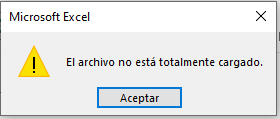
\includegraphics[width=.45\textwidth]{limite.PNG}
\end{figure}
\end{frame}

\begin{frame}
Ahora, hagamos algo más. Pisemos en el botón Aceptar y guardemos como archivo separado por comas (nov2015.csv) y como archivo de Excel (nov2015.xlsx).
\begin{figure}
\centering
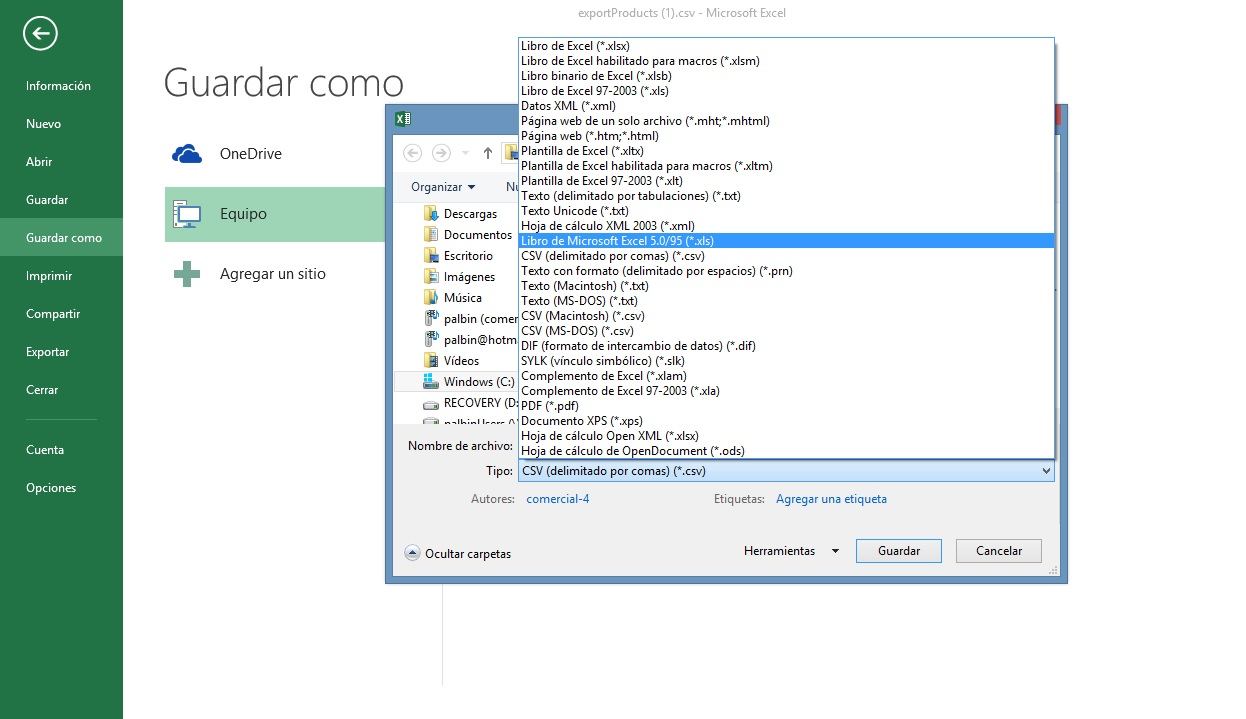
\includegraphics[width=.65\textwidth]{guardarcomo.jpg}
\end{figure}
\end{frame}

\begin{frame}
\begin{figure}
\centering
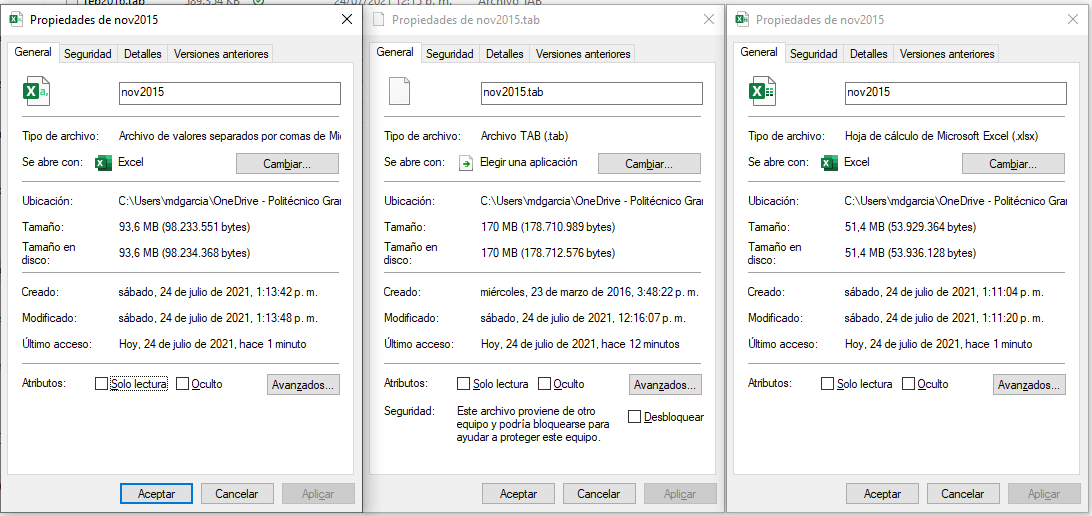
\includegraphics[width=.85\textwidth]{archivos.PNG}
\end{figure}
El archivo .xlsx (51.4MB) no tiene todos los datos que incluye el archivo .tab (170MB) o el archivo .csv (93.6MB).
\end{frame}


\begin{frame}
Al descargar el archivo \textit{Sci-HubRawData.RData} disponible en el mismo enlace anterior \textcolor{blue}{\url{https://osf.io/7gvz2/}} y abrirlo en RStudio, se observará que este archivo .RData (649.5MB) contiene un total de 27.819.966 filas.
\begin{figure}
\centering
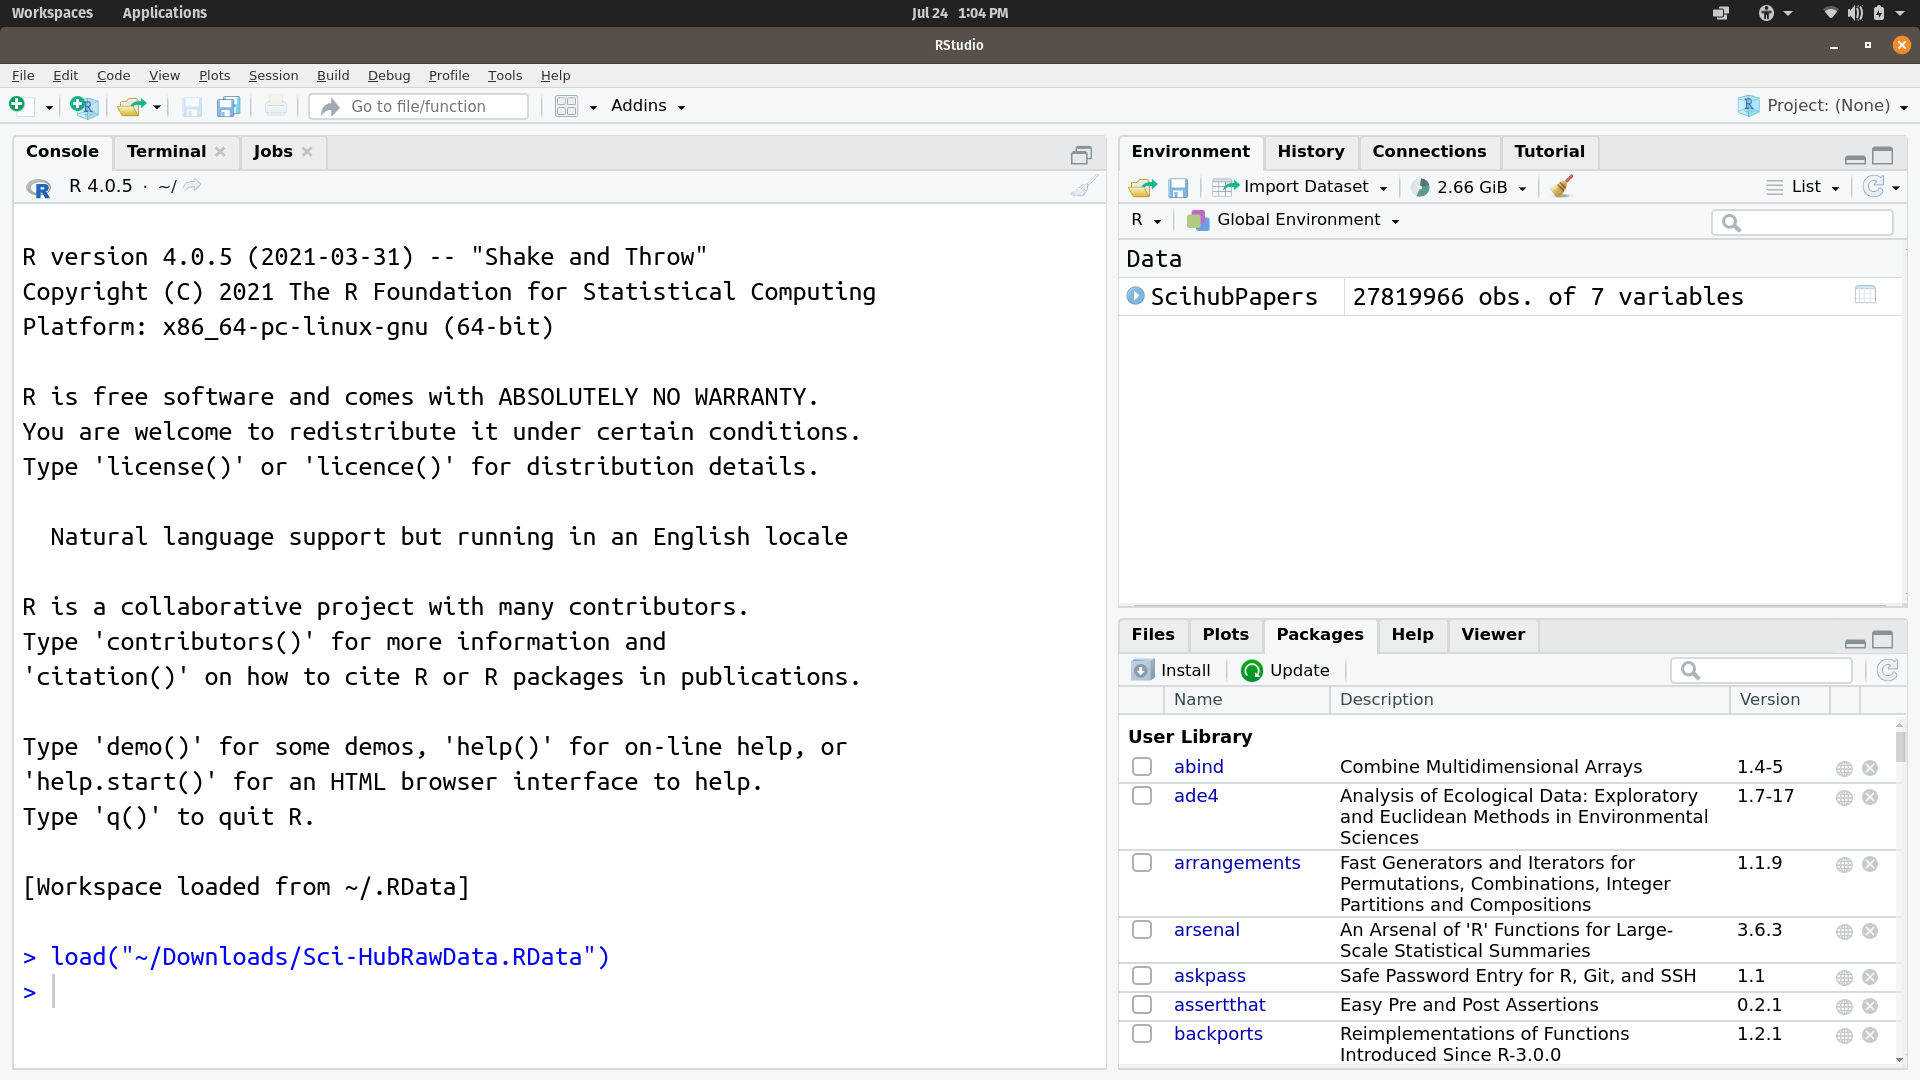
\includegraphics[width=.65\textwidth]{RBigData.png}
\end{figure}
\end{frame}

\begin{frame}
\begin{figure}
\centering

\includegraphics[width=.65\textwidth]{meme.png}
\end{figure}
\end{frame}


\section{Fundamentos de Analítica de Datos}
\begin{frame}
\begin{center}
\Huge
\textcolor{azulcesaclaro}{2\\
--------------------------------\\
Fundamentos de Analítica de Datos}
\end{center}
\end{frame}

\begin{frame}
En la Sesión 3B (slide 12) se describieron algunos de los problemas o deficiencias de las bases de datos del mundo real. En esta sesión vamos a estudiar con detalle algunas de las soluciones más comunes orientadas a resolver estos problemas. Aunque nos apoyaremos en el uso de la librería de Pandas en Python, también se ilustrarán algunos fundamentos con la librería tidyverse en R. 
\begin{figure}
\centering
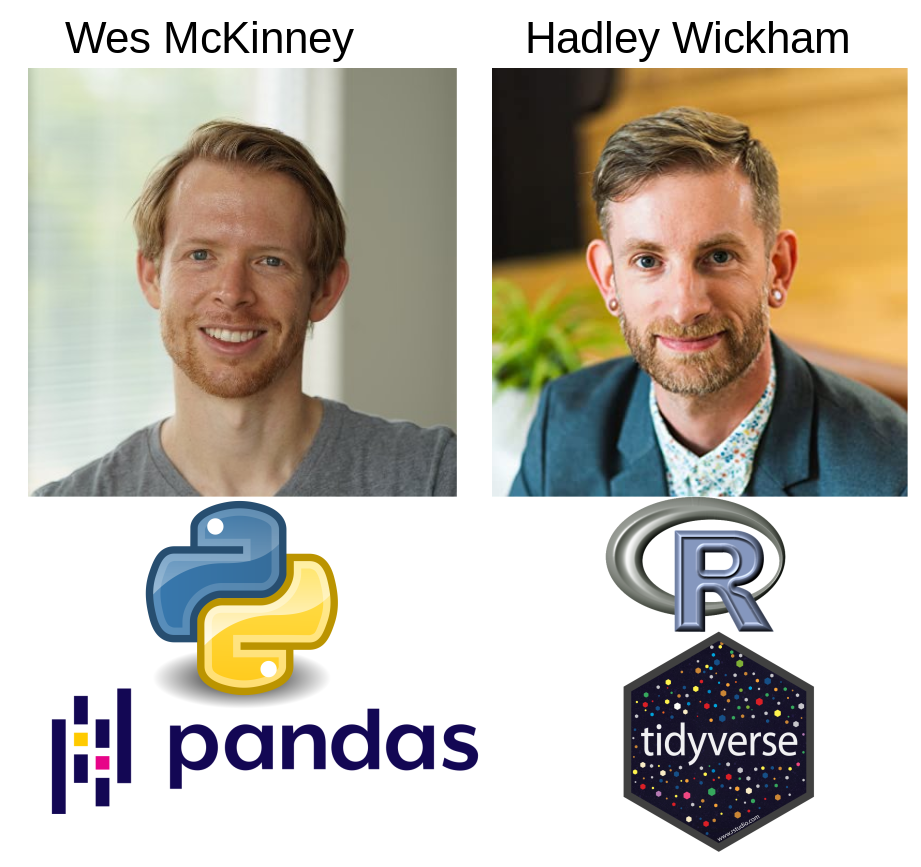
\includegraphics[width=.3\textwidth]{TwoMinds.png}
\end{figure}
\end{frame}

\begin{frame}
En la Sesión 3B (slide 22) nos encontramos con nuestra primera herramienta profesional de la analítica de datos: un archivo jupyter Notebook gestionado desde Anaconda-Navigator.\\
\vspace{0.35cm}
Un archivo jupyter Notebook (.ipynb) es ``como'' un documento de Word. Pero, dentro del .ipynb  podemos incluir códigos de computación. Cuando los códigos son ejecutados, éstos meten dentro del mismo documento el resultado. Mientras que un documento de word (.docx) puede abrirse haciendo doble clic sobre el ícono, para abrir un jupyter Notebook debemos seguir los pasos descritos en la Sesión 3B (slides 19 al 22).\\
\vspace{0.35cm}
Si en este momento, aún no está seguro de cómo abrir exitosamente un archivo .ipynb mejor regrese a la presentación de la Sesión 3B o vuelva a mirar el video de esa clase. Por ahora, no necesitamos aprender los códigos. Abordaremos eso, un poco más adelante y de manera dosificada.
\end{frame}

\begin{frame}
En la Sesión 3B (slide 23) afirmamos que el jupyter Notebook contenía un total de 42 sintaxis de código. Justo antes de cada sintaxis, pueden leerse algunas descripciones verbales (recuadro amarillo) que nos permiten entender qué significan esos códigos (recuadro azul) y comprender el resultado de tales códigos (recuadro rojo).
\begin{figure}
\centering
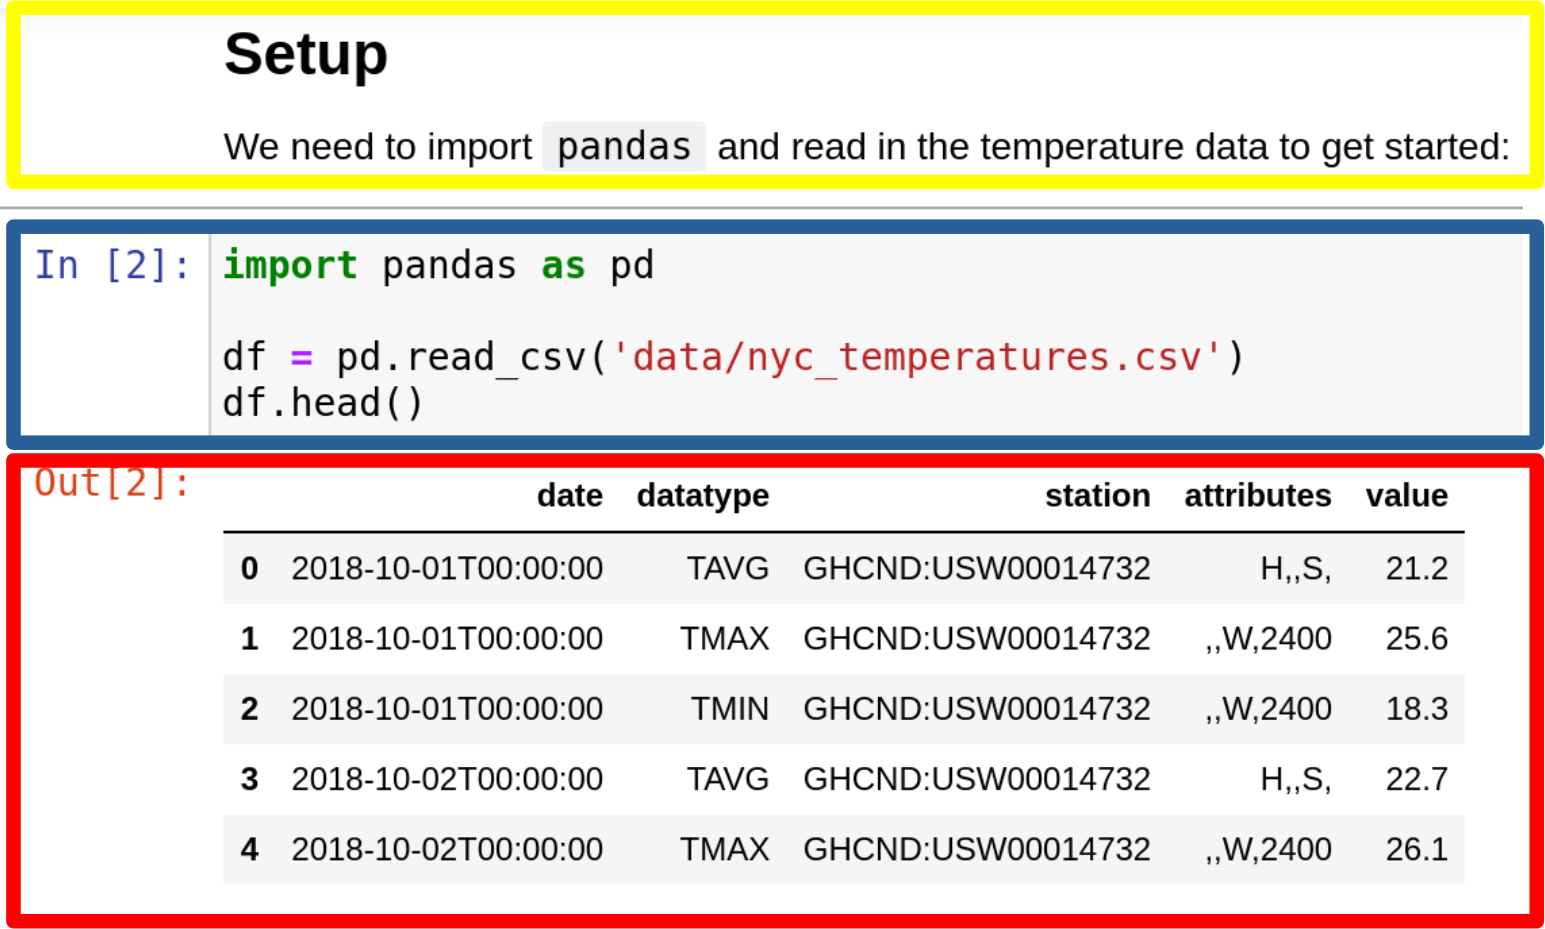
\includegraphics[width=.6\textwidth]{ipynb.png}
\end{figure}
\end{frame}


\subsection{Procedimientos Típicos}
\begin{frame}
\begin{center}
\Huge
\textcolor{azulcesaclaro}{2.1\\
--------------------------------\\
Procedimientos Típicos}
\end{center}
\end{frame}

\begin{frame}
Los procedimientos típicos de la analítica de datos pueden segmentarse en los siguientes tres grandes grupos.
\begin{figure}
\centering
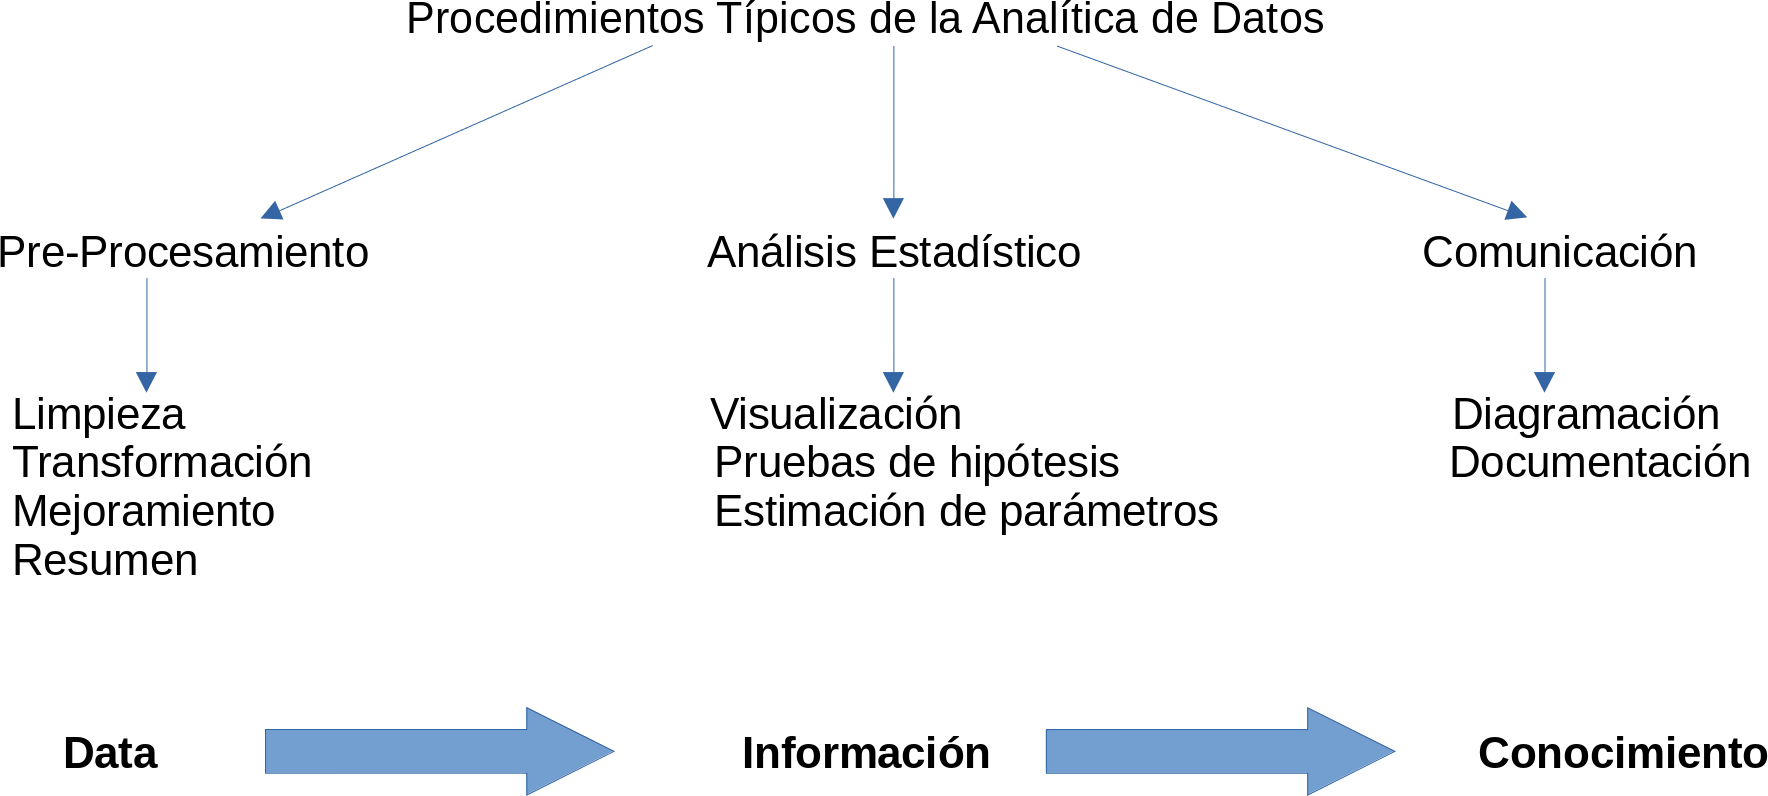
\includegraphics[width=.8\textwidth]{Panorama.png}
\end{figure}
\end{frame}

\begin{frame}
En los capítulos 3 y 4 del libro de texto de \citeauthor{Shmueli2020} \citeyear{Shmueli2020} se abordan los procedimientos típicos de \textbf{Pre-Procesamiento}. También se advierte que los capítulos 5 y 6 abordan los procedimientos de \textbf{Análisis Estadístico} en términos de visualización y algo de prueba de hipótesis (aunque no completamente). Veamos con algún detalle cada uno de los procedimientos típicos para entender cuándo deben aplicarse. Antes de pasar a esto, hace falta resolver una aparente contradicción.
\end{frame}

\begin{frame}
En la Sesión 3B (slide 13), habíamos dicho que una base de datos ordenada era aquella que cumple con las siguientes tres reglas: 1) cada variable ocupa una columna, 2) cada observación ocupa una fila, y 3) cada dato ocupa una celda. Pero... \\
¿Esto no contradice la Figura 3.2 del libro de \citeauthor{Shmueli2020} \citeyear{Shmueli2020}?
\begin{figure}
\centering
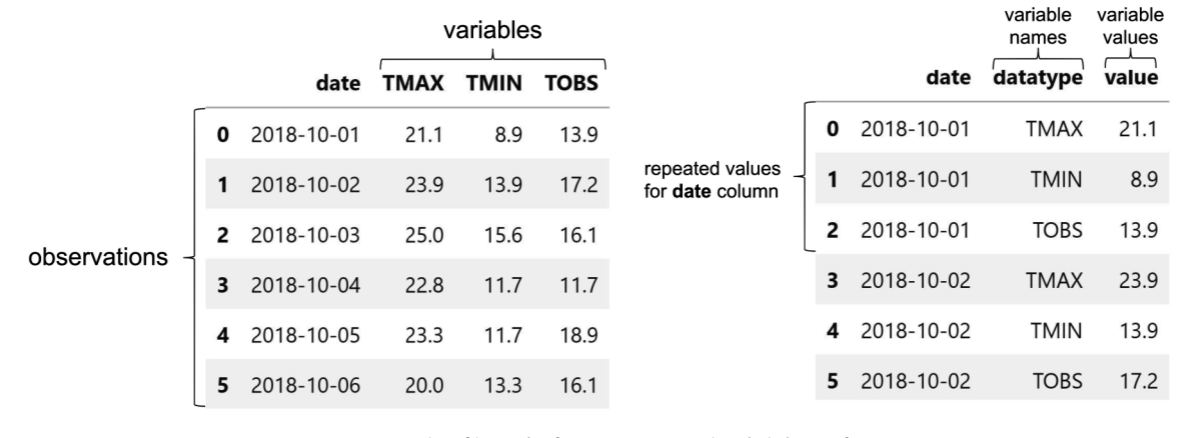
\includegraphics[width=.65\textwidth]{widelong.png}
\end{figure}
\centering
(Izq) base de datos en formato amplio. (Der) base de datos en formato largo.
\end{frame}

\begin{frame}
Las bases de datos en formato amplio son coherentes con las reglas de una base de datos ordenadas presentadas en Sesión 3B (slide 13). Su uso fundamental es para análisis estadísticos.\\
\vspace{0.5cm}
Las bases de datos en formato largo no son coherentes con las reglas mencionadas. Sin embargo, son preferibles cuando se hace minería de datos con \textbf{datos relacionales} (algo que estudiaremos más adelante en la Sesión 8A).
\end{frame}

\begin{frame}
Limpieza (data cleaning):\\
\vspace{0.5cm}
\begin{itemize}
\item Renombrar (renaming): Cuando se necesita cambiar el nombre de una variable (usualmente para poner un nombre más corto).
\item Conversión de tipos (conversion type): Cuando necesitamos cambiar el formato del datos (usualmente de números a fechas)
\item Reordenar, reindexar o sortear (reordering, reindexing, sorting): Cuando se necesita reordenar de menor a mayor o de mayor a menor, o mostrar los valores según un orden específico
\end{itemize}
\end{frame}

\begin{frame}
Transformación (Reshaping data):\\
\vspace{0.5cm}
\begin{itemize}
\item Transponer (Transpose): Cuando debemos intercambiar filas por columnas.
\item Pivotear (Pivot): Cuando queremos pasar una base de datos en formato largo a formato amplio.
\item Licuar (Melting): Cuando queremos pasar una base de datos en formato amplio a formato largo.
\end{itemize}
\end{frame}

\begin{frame}
Mejoramiento: Manejo de datos duplicados, perdidos, o invalidos\\
(Handling duplicate, missing, or invalid data):\\
\vspace{0.5cm}
\begin{itemize}
\item Método \texttt{info()}: Para saber si hay datos perdidos y las columnas tienen el tipo de variable correcto.
\item Método \texttt{isnull() isna()}: Para saber si hay datos nulos o inválidos.
\item Método \texttt{drop\_duplicates()}: Para eliminar registros duplicados.
\end{itemize}
\end{frame}

\begin{frame}
Mejoramiento: Fusionar bases de datos (Merging Data Frames):\\
\vspace{0.5cm}
\begin{figure}
\centering
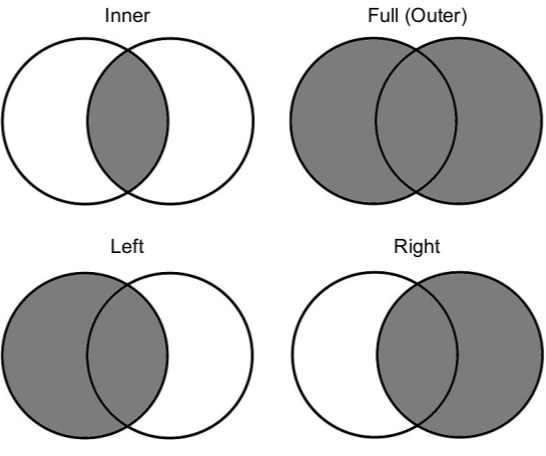
\includegraphics[width=.4\textwidth]{joins.png}
\end{figure}
\centering
(Merge es uno de los más importantes métodos en la analítica de datos)
\end{frame}

\begin{frame}
Mejoramiento: Agregar variables como funciones de variables ya presentes.\\
\vspace{0.5cm}
Mejoramiento: Categorización de valores en una variable\\
\vspace{0.5cm}
Mejoramiento: Aplicación de funciones a grupos de variables\\
\vspace{0.5cm}
Mejoramiento: Cálculos sobre rangos de valores\\
\vspace{0.5cm}\\
Mejoramiento: Aplicación de ``tuberías'' (encadenar varias funciones en un mismo código).\\
\vspace{0.5cm}\\
Mejoramiento: Resumir bases de datos
\end{frame}

\begin{frame}
Si usted ha llegado hasta este punto, ya se encuentra listo para comprender algunos detalles de programación. ¡Incluso si no tiene experiencia programando!\\
\vspace{0.5cm}
En la Sesión 4B se mostrarán algunos trucos para aprender la lógica de la programación de una manera más fácil y sencilla.
\end{frame}

\section*{REFERENCIAS}
\begin{frame}[allowframebreaks]{Referencias}
\tiny{ 
\bibliographystyle{apacite}
\bibliography{REFS.bib}
} 
\end{frame}

\setbeamertemplate{background}{\tikz[overlay,remember picture]\node[opacity=1]at (current page.center){
\includegraphics[width=18cm]{ulam.png}};}
\pgfdeclareimage[height=0cm,width=0cm]{}{}
 \logo{\pgfuseimage{}}
\beamertemplatenavigationsymbolsempty
\begin{frame}
\end{frame}
\end{document}